\documentclass[slidestop,11pt,compress,serif]{beamer} % {{{--

\usepackage{gaelposter}
\geometry{verbose, a4paper, left=0.4cm, right=0.4cm, bottom=2.5cm, top=.8cm}

%\usepackage{relsize} % for relative sizes
\usepackage{graphicx}
\usepackage{multicol}
\usepackage{calc}
\usepackage{enumitem}
% To make enumitem and beamer happy
\newcommand\beameritemnestingprefix{} 

\usepackage{pgf,pgfarrows,pgfnodes}

%%%%%%%%%%%%%%%%%%%%%%%%%% My box command %%%%%%%%%%%%%%%%%%%%%%%
\usepackage{xkeyval}

\makeatletter
\define@key{mybox}{corners}{\def\my@corners{#1}}
\define@key{mybox}{color}{\def\bg@color{#1}}
\define@key{mybox}{width}{\setlength\mybox@width{#1}}
\define@key{mybox}{position}{\def\box@position{#1}}
\define@key{mybox}{innerposition}{\def\box@innerposition{#1}}
\define@key{mybox}{opacity}{\def\box@opacity{#1}}
\define@key{mybox}{height}{\def\box@height{#1}}
\newbox\my@tempbox
\newlength\my@height
\newlength\my@width
\newlength\mybox@width
\newlength\innerbox@width
\newlength\box@heightlgth

\newcommand{\mybox}[2][]{%
  \setlength\mybox@width{\linewidth}%
  \def\box@position{T}%
  \def\box@innerposition{s}%
  \def\box@opacity{0.6}%
  \def\bg@color{gray!25}%
  \def\my@corners{2mm}%
  \let\box@height\@empty
  \setkeys{mybox}{#1}%
  \setlength\innerbox@width{\mybox@width}%
  \advance\innerbox@width by -2mm%
  \setbox\my@tempbox=\hbox{%
  \ifx\box@height\@empty%
    \begin{minipage}{\innerbox@width}%
  \else%
    \setlength\box@heightlgth{\box@height}%
    \advance\box@heightlgth by -\my@corners%
    \advance\box@heightlgth by -1.7ex%
    \begin{minipage}[\box@position][\box@heightlgth][\box@innerposition]%
	    {\innerbox@width}%
  \fi%
      #2%
    \end{minipage}%
  }%
  \my@height=\ht\my@tempbox%
  \my@width=\wd\my@tempbox%
  %
  \advance\my@width by 2mm%
  %
  \begin{minipage}[\box@position]{\mybox@width}%
  \begin{tikzpicture}[rounded corners=\my@corners, fill=\bg@color]
      \fill[fill opacity=\box@opacity, scale=0.5]
      	(-\my@width,-2\my@height) rectangle (\my@width, 2\my@height);
      \path (0,0) node {\box\my@tempbox} ;
  \end{tikzpicture}%
  \end{minipage}%
}
\makeatother

%%%%%%%%%%%%%%%%%%%%%%%%%% Poster related style %%%%%%%%%%%%%%%%%
\newcommand{\vfillll}{\vfilll\vfilll\vfilll\vfilll\vfilll\vfilll\vfilll\vfilll\vfilll\vfilll\vfilll\vfilll\vfilll\vfilll\vfilll\vfilll\vfilll\vfilll\vfilll\vfilll\vfilll\vfilll\vfilll\vfilll\vfilll\vfilll\vfilll\vfilll\vfilll\vfilll\vfilll\vfilll\vfilll\vfilll\vfilll\vfilll\vfilll\vfilll\vfilll\vfilll}

\definecolor{structurecolor}{RGB}{0, 18, 64}

\renewcommand{\section}[1]{%
\vfillll%
\hspace*{-1pt}\mybox[corners=0pt, opacity=0.7, color=structurecolor]{%
{\sffamily\bfseries\Large%
\raisebox{-.4ex}{\rule{0pt}{1ex}}%
\color{white}{#1}}%
}%
\vspace*{1ex}%
}
\renewcommand{\subsection}[1]{%
\normalsize\emph{\sffamily #1\\[-0.9em]\rule{\linewidth}{1pt}}%
\par%
}

\def\name#1{\mbox{\sc #1}}
\setlength\fboxsep{0pt}

\newcommand{\photoframe}[1]{\setlength\fboxsep{0pt}%
\color{gray}\fbox{#1}}

\newcommand{\mydot}{\hspace*{-0.3ex}%
%\raisebox{0.2ex}{\color{structurecolor!50!black}\rule{1.2ex}{1.2ex}}%
\raisebox{0.2ex}{\color{structurecolor}\rule{1.1ex}{1.1ex}}%
\hspace*{0.4ex}%
}

\setitemize{leftmargin=2.5ex}

%%%%%%%%%%%%%%%%%%%%%%%%%%%%%%%%%%%%%%%%%%%%%%%%%%%%%%%%%%%--}}}%
\begin{document}
\newlength\thiscolumnheight

\setbeamertemplate{background}
 {%
\rule{0pt}{0.72\paperheight}%
\centerline{%

\includegraphics[width=0.6\paperwidth]{euroscipy_back}%
}%
}%

\begin{frame}[plain,t]
%%%%%%%%%%%%%%%%%%%%%%%%%%%%%%%%%%%%%%%%%%%%%%%%%%%%%%%%%%%%%%%%%%%%%%%%%%%%%%%%
\sffamily

\centerline{%
\scalebox{2}{\Huge\bfseries EuroScipy 2011}%
}

\smallskip
\centerline{\bfseries\textcolor{structurecolor}{\huge
4\raisebox{.5ex}{\Large th} Annual European Conference for Scientists using Python}}

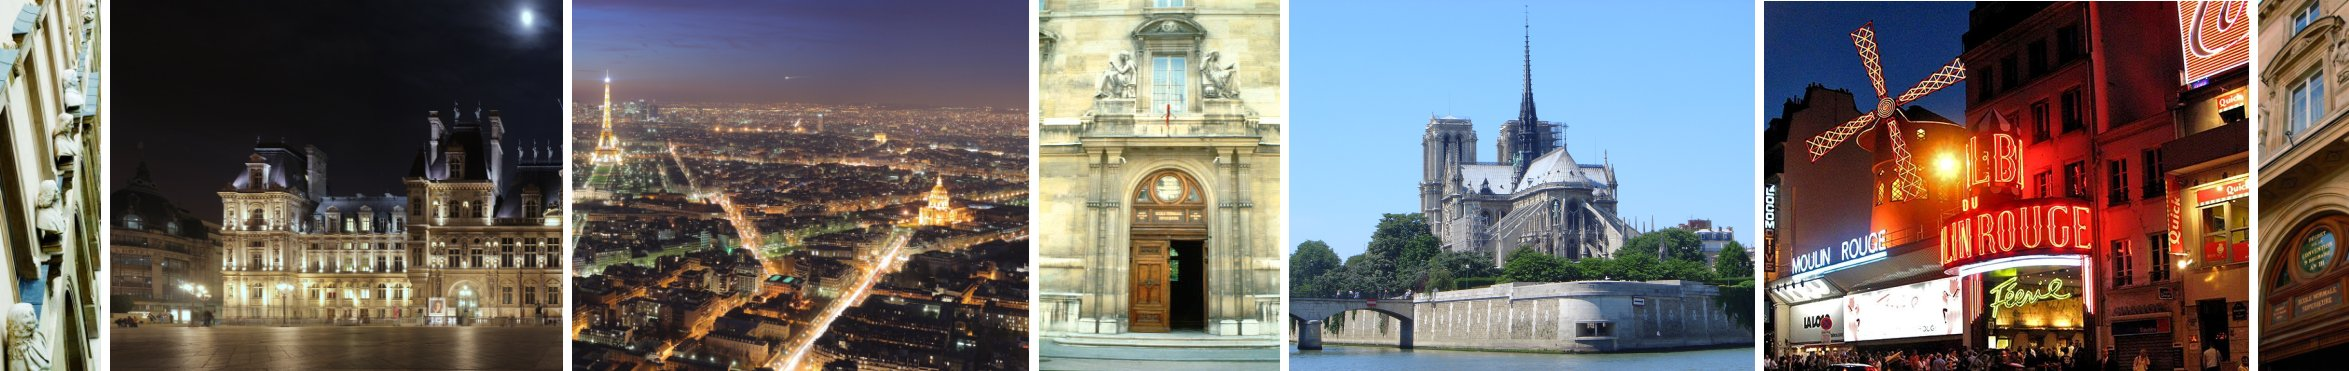
\includegraphics[width=\linewidth]{banner}

\bigskip
\centerline{\bfseries\Huge
Paris, Ecole Normale Supérieure, August 25-28 2011}

\vfillll%

%%%%%%%%%%%%%%%%%%%%%%%%%%%%%%%%%%%%%%%%%%%%%%%%%%%%%%%%%%%%%%%%%%%%%%%%%%%%%%%%
\begin{minipage}{.18\linewidth}
    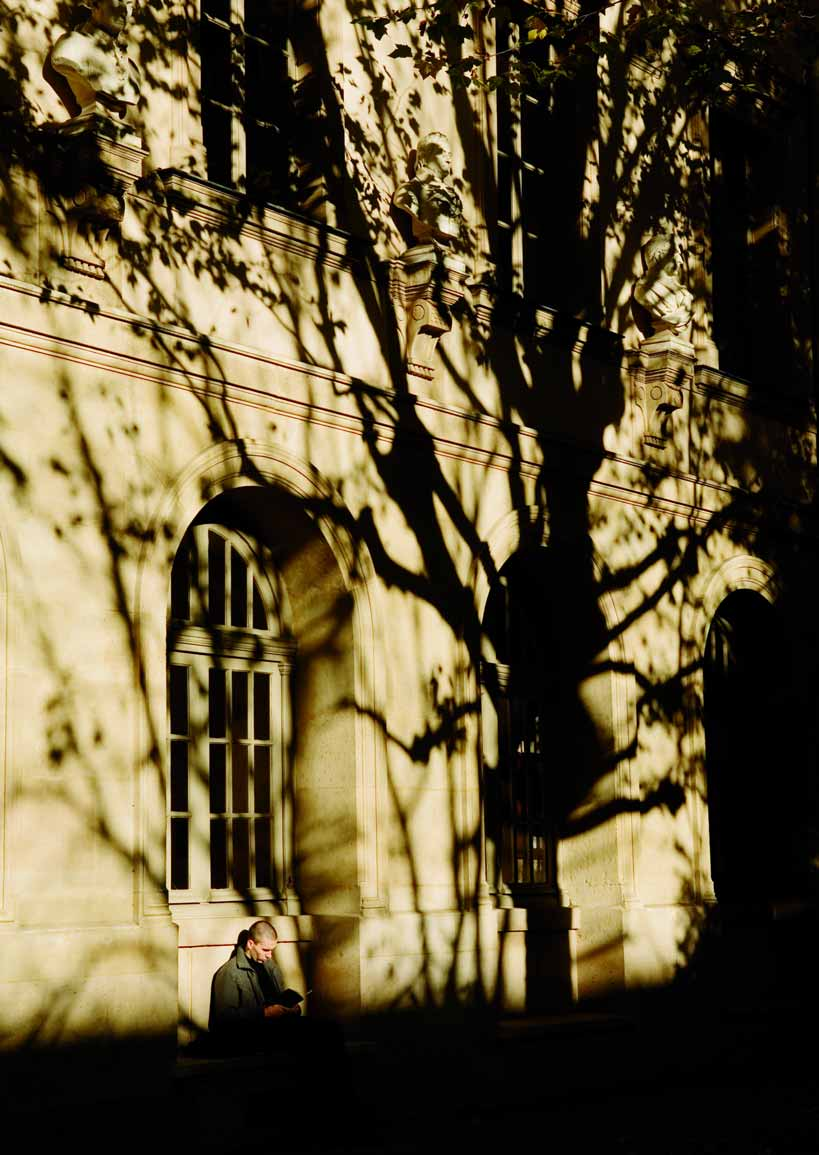
\includegraphics[width=\linewidth]{images/ens-073}

    \bigskip
    \bigskip
    \bigskip
    \bigskip

    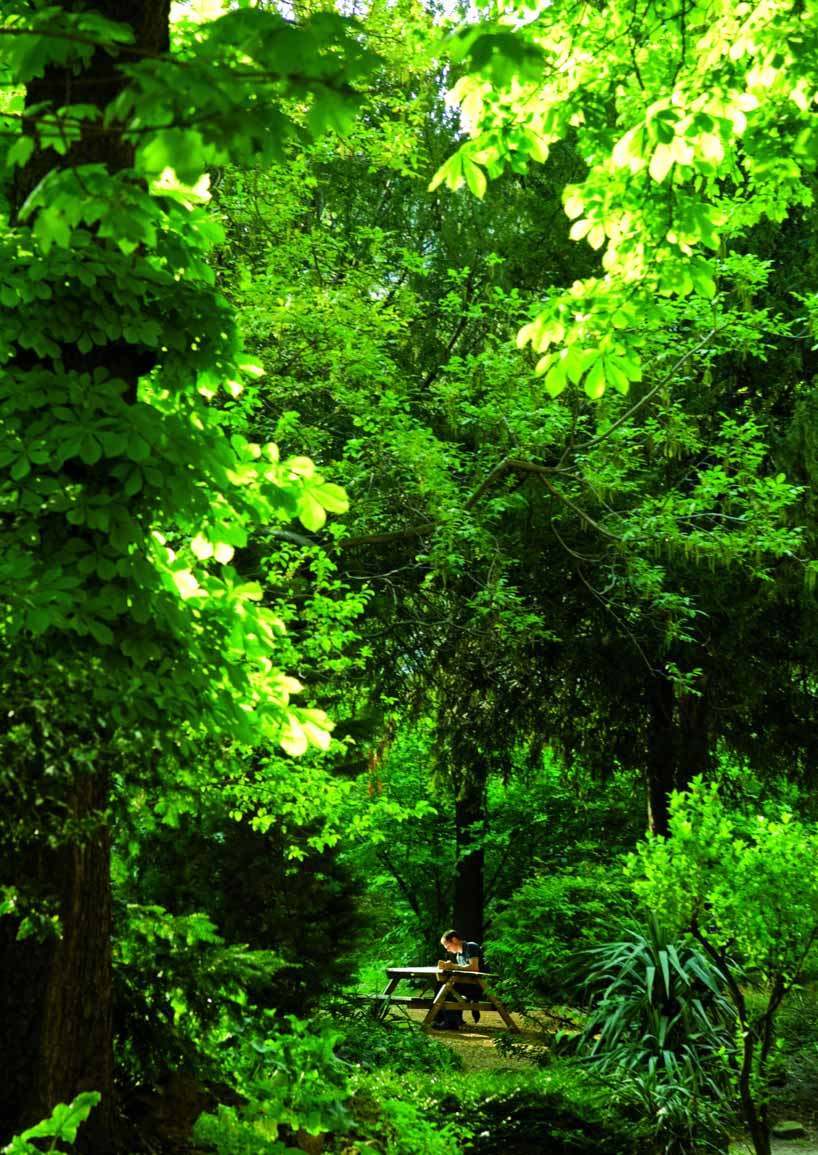
\includegraphics[width=\linewidth]{images/ens-072}

    \bigskip
    \bigskip
    \bigskip
    \bigskip

    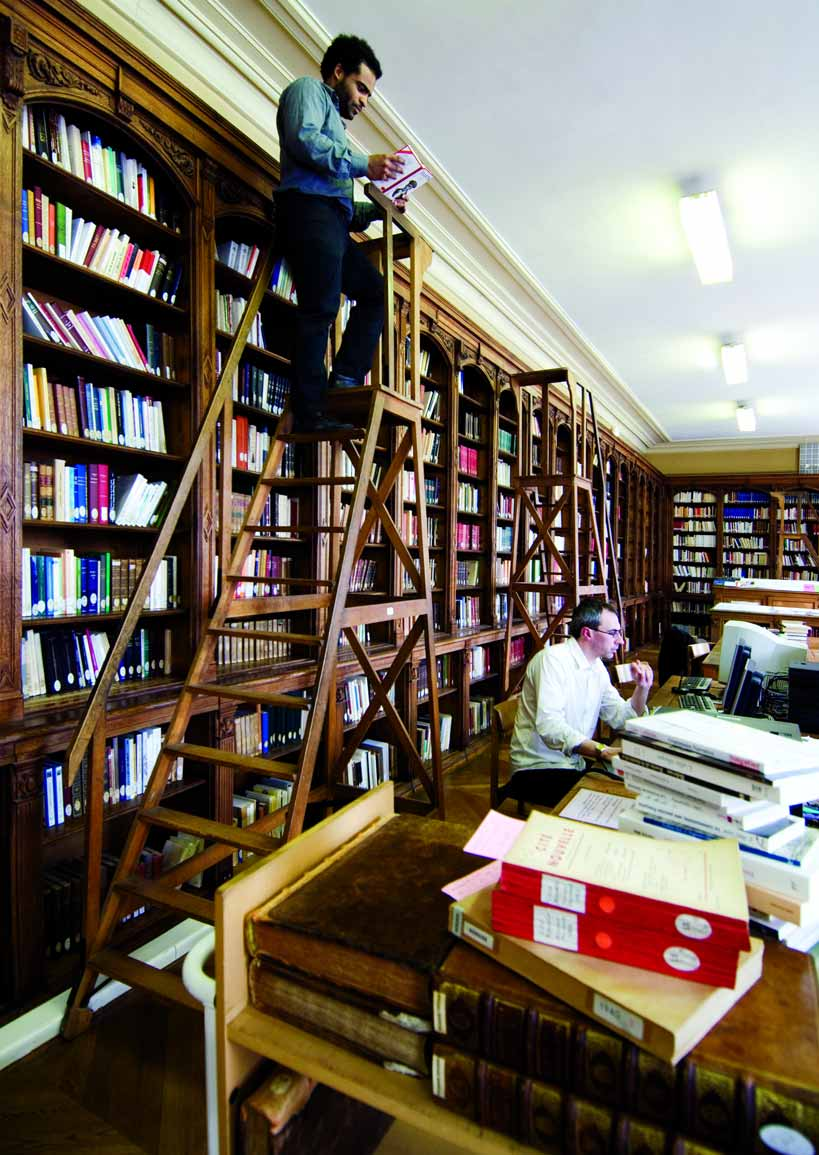
\includegraphics[width=\linewidth]{images/ens-035}
\end{minipage}
%
\hfill
\begin{minipage}{.79\linewidth}


% First row {{{---
%%%%%%%%%%%%%%%%%%%%%%%%%%%%%%%%%%%%%%%%%%%%%%%%%%%%%%%%%%%%%%%%%%%%%%%%%%%%%%%%
\setlength\thiscolumnheight{0.3\textheight} 

%-------------------------------------------------------------------------------
\begin{minipage}[t]{0.49\linewidth}
\section{Dates}%

\vspace*{-1.5ex}%
\mybox[corners=0pt, color=white, width=\linewidth]{
    \large\smallskip

%    \textcolor{structurecolor}{\bfseries Registration opens} \hfill 
%	    Sun. March 29
%
%    \raisebox{.5em}{\textcolor{gray}{\rule{\linewidth}{1pt}}}\\[-.3em]
%    %
    \textcolor{structurecolor}{\bfseries Talk submission deadline} \hfill
	    Sun. May 8

    \raisebox{.5em}{\textcolor{gray}{\rule{\linewidth}{1pt}}}\\[-.3em]
    %
    \textcolor{structurecolor}{\bfseries Program announced} \hfill
	    Sun. May 29

    \raisebox{.5em}{\textcolor{gray}{\rule{\linewidth}{1pt}}}\\[-.3em]
    %
    \textcolor{structurecolor}{\bfseries Tutorials} \hfill
	    Thur. Aug. 25 -- Fri. Aug. 26

    \raisebox{.5em}{\textcolor{gray}{\rule{\linewidth}{1pt}}}\\[-.3em]
    %
    \textcolor{structurecolor}{\bfseries Conference} \hfill
	    Sat. Aug. 27 -- Sun. Aug. 28
    \smallskip
   
}%
\end{minipage}
%
\hfill
%
%-------------------------------------------------------------------------------
\begin{minipage}[t]{0.49\linewidth}
\section{Topics}%

\vspace*{-1.5ex}%
\mybox[corners=0pt, color=white, width=\linewidth]{

    \begin{itemize}
	\item[\mydot] Presentations of scientific tools and libraries using 
	    the Python language, including but not limited to:

	\begin{itemize}
	    \item[\mydot] Vector and array manipulation

	    \item[\mydot] Parallel computing

	    \item[\mydot] Scientific visualization

	    \item[\mydot] Scientific data flow and persistence

	    \item[\mydot] Algorithms implemented or exposed in Python

	    \item[\mydot] Web applications and portals for science and 
	    engineering
	\end{itemize}

	\item[\mydot] Reports on the use of Python in scientific achievements 
	or ongoing projects.

	\item[\mydot] General-purpose Python tools of
	interest to the scientific community.
    \end{itemize}

}%
\end{minipage}
% ---}}}

%\vspace*{1cm}

% Second row {{{---
%%%%%%%%%%%%%%%%%%%%%%%%%%%%%%%%%%%%%%%%%%%%%%%%%%%%%%%%%%%%%%%%%%%%%%%%%%%%%%%%
\setlength\thiscolumnheight{0.3\textheight} 

%-------------------------------------------------------------------------------
\begin{minipage}[t]{0.49\linewidth}
~

\rule{0pt}{3.5cm}

\section{Preliminary program}%

\vspace*{-1.5ex}%
\mybox[corners=0pt, color=white, width=\linewidth]{

    \subsection{2 days introductory tutorial}
    \large
    Getting up to speed with Python for scientific computing.

    \subsection{Advanced tutorials}
    Experts presenting top-notch libraries: visualization, advanced array
    manipulation, symbolic algebra, packaging, sparse matrix computing, C
    binding, cython.

 %   {\bfseries \mbox{R. Cimrman}, \mbox{F. Pedregosa}, \mbox{M. Poinot}, 
%    \mbox{G. Varoquaux}, \mbox{P. Virtanen}, \mbox{T. Ziade}...}

    \subsection{Keynote speakers}

    {\bfseries Marian Perte}

    {\normalsize \textcolor{structurecolor}{Open University, Director of the 
    Center for Research in Computing}
    %
    Empirical Studies of Software Development}

    {\bfseries Fernando Perez}

    {\normalsize \textcolor{structurecolor}{UC Berkeley, Helen Wills
    NeuroScience Institute}
    %
    Author of {\sl IPython}.}
}%
\end{minipage}
%
\hfill
%
%-------------------------------------------------------------------------------
\begin{minipage}[t]{0.49\linewidth}
~

\rule{0pt}{.1cm}

\section{Committees}%

\vspace*{-1.5ex}%
\mybox[corners=0pt, color=white, width=\linewidth]{
    \smallskip
    \subsection{Conference chairs}
	\large

	\vspace*{-1ex}
	\begin{itemize}
	    \item[\mydot] Gaël Varoquaux {\small (INSERM/INRIA)}

	    \item[\mydot] Nicolas Chauvat {\small (Logilab)}
	\end{itemize}

    \subsection{Program committee}

	\vspace*{-1ex}
	\begin{itemize}
\item[\mydot] Chair: Tiziano Zito {\small (TU Berlin)}
             
\item[\mydot] Romain Brette {\small (ENS Paris)}
             
\item[\mydot] Emmanuelle Gouillart {\small (Saint-Gobain Research)}

\item[\mydot] Eric Lebigot {\small (Laboratoire Kastler Brossel)}
             
\item[\mydot] Konrad Hinsen {\small (Soleil Synchrotron)}
             
\item[\mydot] Hans Petter Langtangen {\small (Simula laboratories)}

\item[\mydot] Jarrod Millman {\small (UC Berkeley)}
             
\item[\mydot] Mike Müller {\small (Python Academy)}
             
\item[\mydot] Didrik Pinte {\small (Enthought Inc)}

\item[\mydot] Marc Poinot {\small (ONERA)}
             
\item[\mydot] Christophe Pradal {\small (CIRAD/INRIA)}
             
\item[\mydot] Andreas Schreiber {\small (DLR)}

\item[\mydot] Stéfan van der Walt {\small (University of Stellenbosch)}
    \end{itemize}
}%
\end{minipage}
% ---}}}

\end{minipage}
%%%%%%%%%%%%%%%%%%%%%%%%%%%%%%%%%%%%%%%%%%%%%%%%%%%%%%%%%%%%%%%%%%%%%%%%%%%%%%%%

\vfillll%


%%%%%%%%%%%%%%%%%%%%%%%%%%%%%%%%%%%%%%%%%%%%%%%%%%%%%%%%%%%%%%%%%%%%%%%%%%%%%%%%
% Logos {{{---
\begin{minipage}{.25\linewidth}
    
\includegraphics[height=1.2cm]{logilab}
\end{minipage}
\hfill
\begin{minipage}{.4\linewidth}
    \centerline{\bfseries\textcolor{structurecolor}{\huge
			\url{http://www.euroscipy.org}}}
\end{minipage}
\hfill
\begin{minipage}{.25\linewidth}
    \hfill
\includegraphics[height=1cm]{logo_inria_simple}%
\end{minipage}

\vskip 1cm
\vfill\vbox{}%
%%%%%%%%%%%%%%%%%%%%%%%%%%%%%%%%%%%%%%%%%%%%%%%%%%%%%%%%%%%%%%%%%%%%%%%%%%%%%%%%
% ---}}}


%%%%%%%%%%%%%%%%%%%%%%%%%%%%%%%%%%%%%%%%%%%%%%%%%%%%%%%%%%%%%%%%%%%%%%%%%%%%%%%%
\end{frame}
\end{document}
